%%%%%%%%%%%%%% COPYRIGHT INFORMATION %%%%%%%%%%%%%%
% Template by
% Author: Sascha Frank 
% Nov. 2006
% University Freiburg 
% www.informatik.uni-freiburg.de/~frank/
% Distributed freely for non-commercial use

%%%%%%%%%%%%%%%%%%%%% PREAMBLE %%%%%%%%%%%%%%%%%%%%%
\documentclass{beamer}
\usepackage{beamerthemeshadow}
\usepackage{lmodern}

%%%%%%%%%%%%%%%%%%%%% DOCUMENT %%%%%%%%%%%%%%%%%%%%%
\begin{document}
\title{Movie-Chain-Runner Problem}
\author[Singh,Zong]{Shashank Singh \and Jimmy Zong}
\date{\today} 

\frame{\titlepage}

\frame{\frametitle{Outline}\tableofcontents}

\section{Team Members}
\frame{\frametitle{Team Members}
\begin{itemize}
\item Sung Uk Ryu
\item Eugene Scanlon
\item Shashank Singh
\item Jimmy Zong
\end{itemize}
}

\section{Problem Introduction}
\frame{\frametitle{The Problem}
\begin{block}{The Problem}
Find the ``longest'' list of overlapping titles in a list of movie titles.
\end{block}

\pause
For Example: In the list
\begin{itemize}
\item Day of the Dead
\item Live and Let Die
\item Dead Poets' Society
\item Die Another Day
\item The Last Samurai
\end{itemize}
the ``longest'' chain is
\begin{center}
``Live and Let Die Another Day of the Dead Poets' Society.''
\end{center}
}

\frame{\frametitle{The Problem}
\begin{itemize}
\item Equivalent to finding a Longest Simple Path in a directed graph
\pause
\item The Longest Path Problem is NP-Complete
\end{itemize}
}

\frame{\frametitle{Previous Attempts}
\begin{itemize}
\item Summer 2010   --  255 titles
\item Fall 2010     --  271 titles (845 words)
\item Summer 2011   --  311 titles (997 words)
\item Fall 2011     --  323 titles (1030 words)
\item Spring 2012   --  327 titles (1055 words)
\end{itemize}
}

\section{Benefits}
\frame{\frametitle{Benefits}
Our group will gain experience
\begin{itemize}
\item programming in Python (and maybe C, MATLAB, or another language)
\item working as a group toward a common goal
\item handling and processing a large data set
\item implementing graph algorithms
\item designing and implementing approximation algorithms for an NP-hard problem
\end{itemize}
}

\section{Approach}
\frame{\frametitle{Approach}
\begin{itemize}
\item Algorithms
\item Project Timeline (Gantt Chart)
\end{itemize}
}

\subsection{Algorithms}
\frame{\frametitle{Algorithms}
\begin{enumerate}
\item Brute Force (247 titles so far)
\end{enumerate}
}

\subsection{Project Timeline}
\frame{\frametitle{Gantt Chart}
\begin{center}
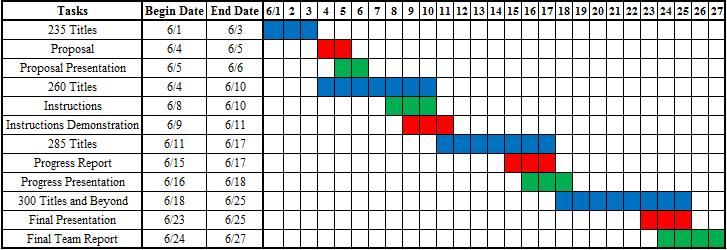
\includegraphics[scale=0.45]{gantt}
\end{center}
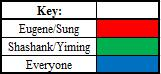
\includegraphics[scale=0.5]{ganttLegend}
}

\section{Evaluation}
\frame{\frametitle{Evaluation}
\begin{enumerate}
\item Length of the longest chain we find
\item Compare performance of a few different algorithms
\item Predict runtime for entire computation by solving tractable subproblems
\end{enumerate}
}

\section{Qualifications}
\frame{\frametitle{Qualifications}
\begin{itemize}
\item Sung Uk Ryu
\item Eugene Scanlon
\end{itemize}
}

\frame{\frametitle{Qualifications}
\begin{itemize}
\item Shashank Singh
\begin{itemize}
\item Senior CS/Math Dual Degree
\item Completed undergrad CS/Math curricula, including courses specifically in
Data Structures/Algorithms and Discrete Math (15-121, 15-211, 15-251, 15-451,
21-301, 21-484)
\item TA'd 15-211 and 15-251
\item Have extensive experience analyzing large data sets for research
\end{itemize}
\item Jimmy Zong
\begin{itemize}
\item Sophomore CS major
\item Completed 15-112, \ldots
\item Done \ldots projects
\end{itemize}
\end{itemize}
}

\section{Summary}
\frame{\frametitle{Summary}\tableofcontents}

\frame{\frametitle{Sources}
\begin{itemize}
\item Gantt Chart created using software from the Gantt Project
\begin{itemize}
\item http://www.ganttproject.biz/ (accessed June 4, 2013)
\end{itemize}
\end{itemize}
}
\end{document}
